\documentclass[border=10pt]{standalone}
\usepackage{pgfplots}
\pgfplotsset{compat=1.17}
\begin{document}
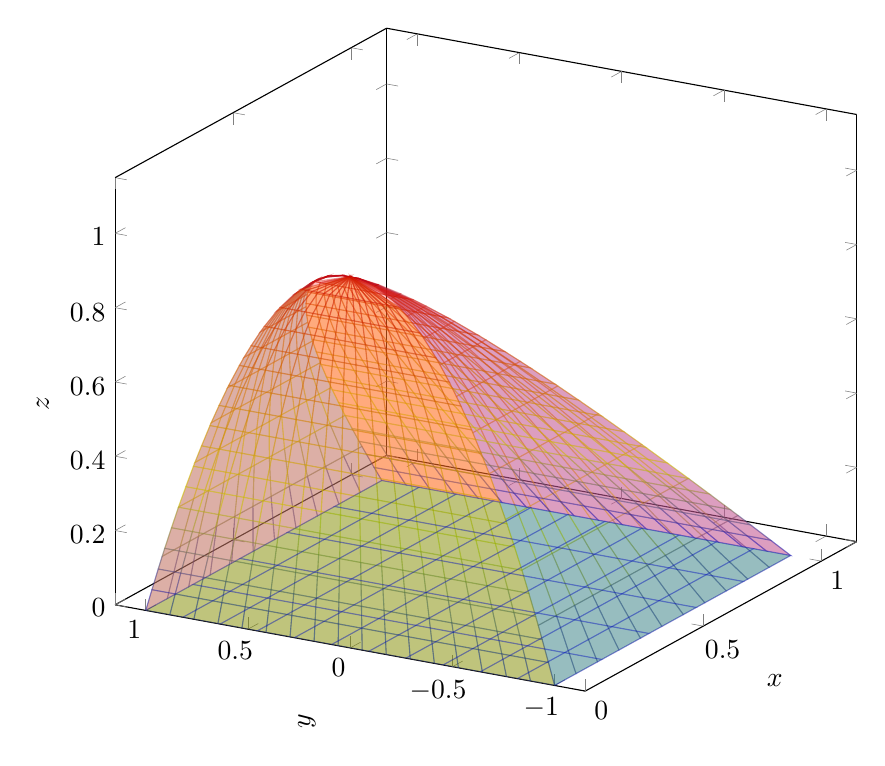
\begin{tikzpicture}
\begin{axis}[
    width=11cm, height=10cm,
    view={-60}{22},
    xlabel=$x$, ylabel=$y$, zlabel=$z$,
    xmin=0, xmax=1.15, ymin=-1.15, ymax=1.15, zmin=0, zmax=1.15,
    axis lines=box]
% Parabolic cylinder z = 1 - y^2 (portion with 0 <= x <= y^2)
\addplot3[surf, shader=faceted, opacity=0.35, color=blue!60,
    domain=0:1, domain y=-1:1, samples=12, samples y=26]
    ({y^2*x}, {y}, {1-y^2});
% Plane x + z = 1  (front face)
\addplot3[surf, shader=faceted, opacity=0.35, color=red!70,
    domain=0:1, domain y=-1:1, samples=18, samples y=18]
    ({x}, {sqrt(x)*y}, {1-x});
% Plane x = 0 (back face)
\addplot3[surf, shader=faceted, opacity=0.35, color=orange,
    domain=0:1, domain y=-1:1, samples=18, samples y=18]
    ({0}, {sqrt(1-x)*y}, {x});
% Plane z = 0 (bottom)
\addplot3[surf, shader=faceted, opacity=0.25, color=green!60!black,
    domain=0:1, domain y=-1:1, samples=6, samples y=12]
    ({x}, {y}, {0});
\end{axis}
\end{tikzpicture}
\end{document}
